The main goals of the \hbox{\emph{Track Me}}'s system are to provide to the third parties a big pool of users from wich can gather data (offered by the base service of D4H) and to provide to the users a timely medical  assistance in case of illness (offered by the SOS service on top of D4H). The system is designed to be used as two different application: one for users and one for third parties. The users' application sends data about them to \hbox{\emph{Track Me}}'s servers where then they can be collected by third parties throught theirs application by making a request for receiving data of a specific users or anonimized data of multiple users. \hbox{\emph{Track Me}} uses user's data also for garanting a timely medical assistance to the users who have activated the ASOS service in case of drop of theirs healt parameters gathered by theirs application by contacting an external SOS service.\\

The following diagram is provided to better describe the Track Me's system:

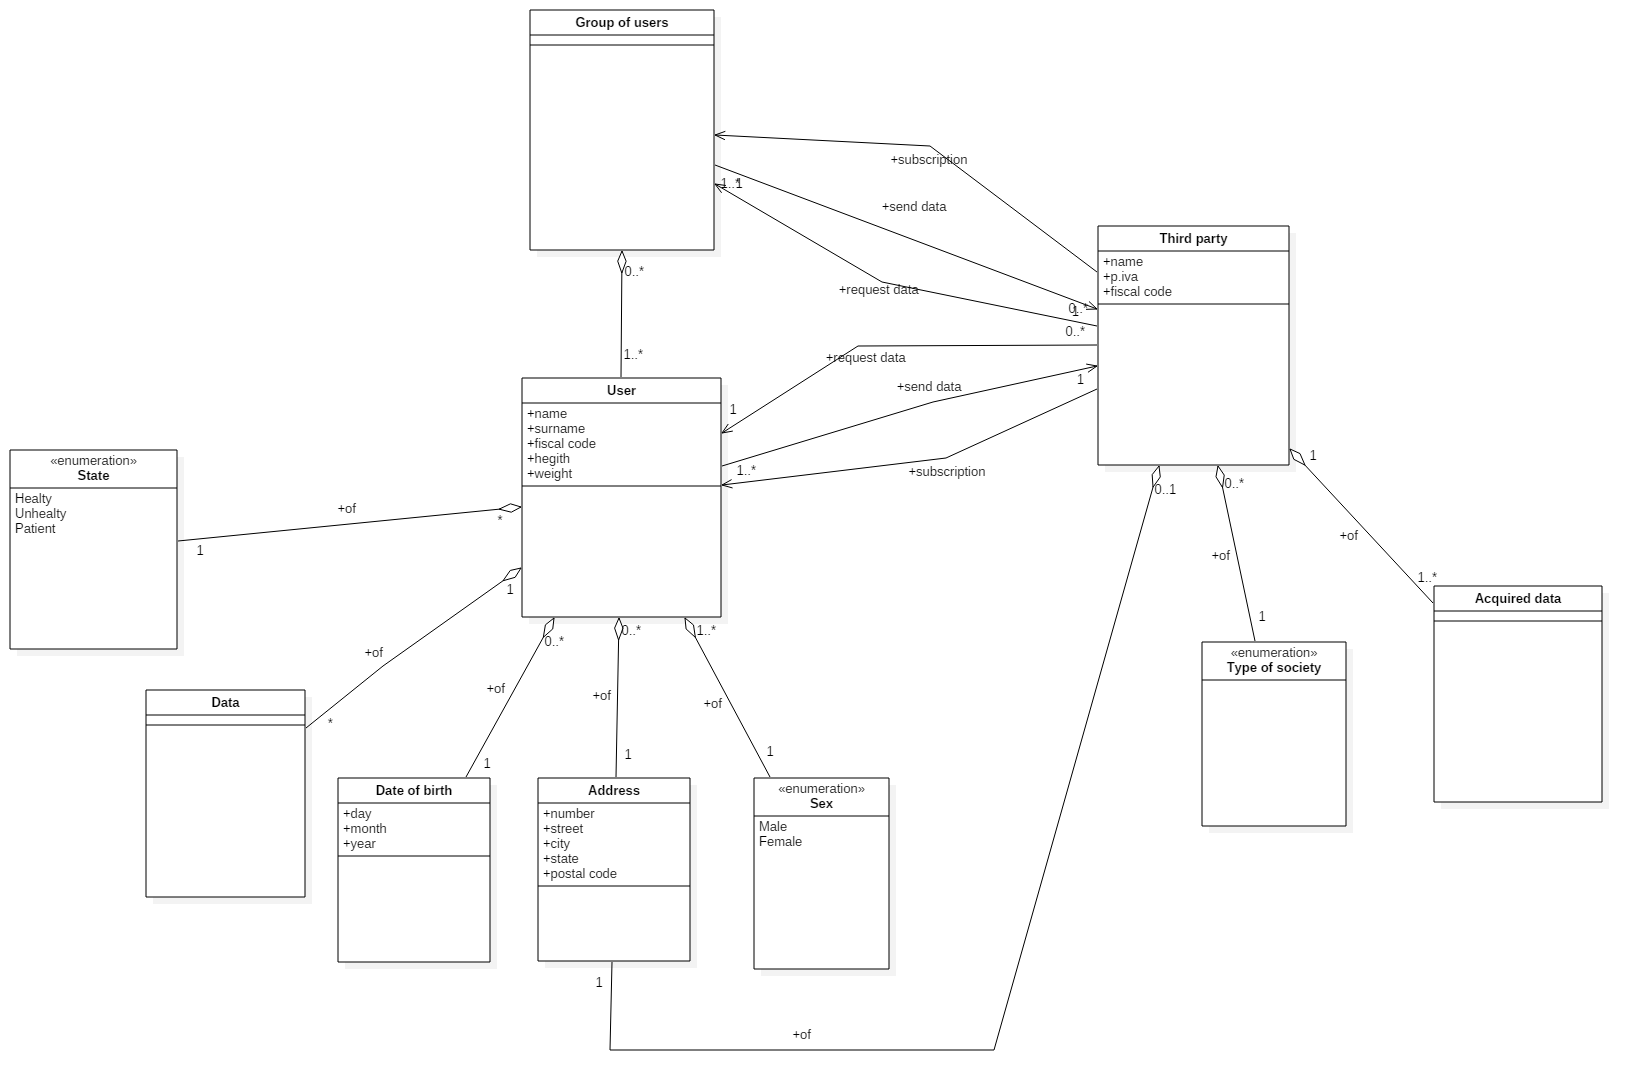
\includegraphics[width=1.00\textwidth]{./pictures/uml_v1.png}\par

As shown, all the system is centered on garanting data to third parties of users or groups of users and garanting medical assistance for the users who have activated the SOS service (the attribute "state" of the user is intended right for this scope).